\newpage
% Heap
\section{Heap}

% Heap Introduction
To model the memory used by the program we want to verify, we use a graph with nodes and labeled edges.
Each node represents a memory cell whereas each edge represents a pointer to the next part of the Data-Structure.
The edges are labeled with a color to distinguish between these selectors. For simplicity only structures with
two pointers will be considered. The selectors will be labeled 1 and 2 
(instead of common known selectors \textit{next} and \textit{prev}). The approach we use though can be generalized
for structures with any number of selectors.\\
We now need to define two special nodes, one for the \textit{null pointer} and one for \textit{dangling pointers}.
The \textit{null node}, written as $\#$, will be used to model null successors whereas the \textit{dangling node},
written as $*$, will be used to model pointers which used to point to memory that has been either freed or not yet been allocated.
Both these nodes will be used by making the corresponding edge link to one of them.\\
In addition, we need to model a program variable by labeling the node the variable points to, with the variable's name.\\
The above leads to the following formal definition of a \textit{heap}.\\
Let $C = \{1,2\}$ be a set of colors and $X$ be a set of program variables.\\

% Heap Definition
$heap = (\overline{M}, E, s, t, \tau, \lambda)$ where:

\begin{itemize}
	\item $\overline{M} = M \cup \{\#,*\}$ represents the finite set of allocated memory cells, together with the two special nodes 
		representing the null value and the dangling pointer, respectively.
	\item $E$ is a finite set of edges.
	\item The source function $s : E \rightarrow M$ is a total function that gives the source of the edges.
	\item The target function $t : E \rightarrow M$ is a total function that gives the target of the edges.
	\item The type function $\tau : E \rightarrow C$ is a total function that gives the color of the edges.
	\item $\lambda : X \rightarrow M$ is a total function that defines the positions of the program variables.
\end{itemize}

% TODO: References
\noindent
% Heap Invariant
To verify that each memory cell has exactly one outgoing edge labeled 1 and one outgoing edge labeled 2, the heap must satisfy
the following invariant:\\

$\forall c \in C$ $\forall m \in M : |s^{-1}(m) \cap \tau^{-1}(c)| = 1$ \\

\noindent
% Heap operations
\subsection{Operations on Heaps}
To work with these heaps, we have to define two operations on it. \\
Let $h = (\overline{M}, E, s, t, \tau, \lambda)$ be a heap, 
then $h \oplus m$ is equal to $h'$ for $m \in M$, where $h'$ is the heap resulting from the addition of the cell $m$ and it's two
outgoing \textit{dangling} edges.\\
Respectively $h \ominus m$ is defined as the heap $h'$ with the cell $m$ and it's outgoing edges removed, where
all edges that previously pointed to $m$ are now \textit{dangling} edges.
% TODO: Formal Definition if enough space left

\newpage
% Signatures
\section{Signatures}
We now define a way to characterize heaps into classes with certain properties.
Therefore we introduce Signatures, which can be seen as a predicate describing a set of minimal
conditions a heap has to fulfill to satisfy the predicate. 
Intuitively a signature can be viewed as a heap with some parts "missing". 
% TODO: Reference!

\noindent
We define Signatures as a tuple $(\overline{M}, E, s, t, \tau, \lambda)$ identically to heaps with the exception,
that the functions $\tau$ and $\lambda$ can be partial. As for the heaps, we also define two invariants for
signatures:

% Signature Invariants
\begin{enumerate}
	\item $\forall c \in C$ $\forall m \in M : |s^{-1}(m) \cap \tau^{-1}(c)| \le 1$
	\item $\forall m \in M : |s^{-1}(m)| \le 2$
\end{enumerate}

\noindent
The first invariant states, that each signature's memory cell can't have more than one outgoing edge of each color.
Whereas the second invariant states, that each memory cell can have at most two outgoing edges in total.

\subsection{Operations on Signatures}
As we did for the heaps, we define operations for signatures. Since signatures are basically heaps, we
can carry over the definition of $\ominus$.\\
Let now $sig = (\overline{M}, E, s, t, \tau, \lambda)$ be a signature. 
We define $sig \boxminus e$ as the signature $sig'$ where $e \in E$ has been removed from $sig$ and it's functions 
$s$, $t$ and $\tau$ are restricted to $E' = E\setminus\{e\}$. We define the addition of an edge in a similar way.
Given $m_1 \in M$, $m_2 \in \overline{M}$ and $c \in C$, $sig \boxplus (m_1 \xrightarrow{c} m_2)$ denotes the addition
of a transition of color $c$ between $m_1$ and $m_2$ to $sig$. We conclude with the definition for the Addition of
a memory cell $m \not\in \overline{M}$ as follows: $sig.(\overline{M} := \overline{M} \cup {m})$ equals the Signature
$sig' = (\overline{M} \cup {m}, E, s, t, \tau, \lambda)$.

\subsection{Ordering on Signatures}

To define an ordering on signatures, we need to take a look at the following five $ordering$ $steps$ and how they are defined first.
We begin with the definition of $unlabeled$, $isolated$ and $simple$ memory cells.
Given a Signature $sig = (\overline{M}, E, s, t, \tau, \lambda)$ and a cell $m \in \overline{M}$, $m$ is $unlabeled$ if 
$\lambda^{-1}(m) = \emptyset$. We say the cell is $isolated$, if it is $unlabeled$ and also $s^{-1}(m) = \emptyset$ and 
$t^{-1}(m) = \emptyset$ hold. The cell $m$ is called $simple$, when $m$ is $unlabeled$ and the following constraints
hold: $s^{-1}(m) = \{e_1$\}, $t^{-1}(m) = \{e_2\}$, $e_1 \not= e_2$ and $\tau(e_1) = \tau(e_2)$. 
We can now define an ordering on two given signatures $sig_1 = (\overline{M}_1, E_1, s_1, t_1, \tau_1, \lambda_1)$ and
$sig_2 = (\overline{M}_2, E_2, s_2, t_2, \tau_2, \lambda_2)$, written as $sig_1 \vartriangleleft sig_2$ if $sig_1$ results
from the application of one of the following operations:

\begin{itemize}

	\item $Isolated$ $cell$ $deletion$. There is an isolated $m \in M_2$ s.t. $sig_1 = sig_2 \ominus m$.
	\item $Edge$ $deletion$. There is an edge $e \in E_2$ such that $sig_1 = sig_2 \boxplus e$.
	\item $Contraction$. There is a simple cell $m \in M_2$, edges $e_1,e_2 \in E_2$ with $t_2(e_1) = m$,
		  $s_2(e_2) = m$, $\tau(e_1) = \tau(e_2)$, and $sig_1 = sig_2.t[e_1 \mapsto t(e_2)] \ominus m$. 
	\item $Edge$ $decoloring$. There is an edge $e \in E_2$ such that $sig_1 = sig_2.\tau[e \mapsto \bot]$
	\item $Label$ $deletion$. There is a label $x \in X$ such that $sig_1 = sig_2.\lambda[x \mapsto \bot]$

\end{itemize}
% TODO: Reference!



\subsection{Transition}





\section{Monotonic Abstraction}

\subsection{Computing Predecessors}

\subsection{Correctness of pre?}

\section{The Reachability Algorithm}



\begin{comment}
This section concerns the main topic. In the following you can see a
small illustration of how to use itemizings and enumerations.


\begin{itemize}
	\item Point 1.
	\item Point 2.
\end{itemize}

\begin{enumerate}
	\item Point 1.
	\item Point 2.
	\begin{enumerate}[I)]
  \item Point 1.
  \item Point 2.
\end{enumerate}
\end{enumerate}

\begin{enumerate}
	\item Point 1.
	\item Point 2.
\end{enumerate}

\begin{description}
	\item[Term one: ] Description of term one.
	\item[Term two: ] Description of term two.
\end{description}

In Algorithm~\ref{alg:nameOfAlgorithm} you can see how we define an
algorithm.

\begin{Algorithm}
	\caption{Describe the purpose of the algorithm. For more 
	information see the \href{../manuals/newalg.pdf}{newalg-
	Manual}.}
	\label{alg:nameOfAlgorithm}
	\begin{algorithm}{\text{void method}}{\text{typeA argumentA, 
												typeB argumentB}}
		\text{write the algorithm in pseudocode} \\
		\text{it should not go into detail, but display main idea} \\
		\text{however, keep being consistent} \\
		x\=1\text{ (this is how to assign a value to a variable)} \\
		\begin{WHILE}{\text{a condition being True or False}}
			\text{do something} \\
			\text{and something else} \\
		\end{WHILE} \\
		\begin{IF}{\text{a condition being True or False}}
			\text{point }1 \\
		\ELSE
			\begin{IF}{\text{another condition}}
				\text{point }2 \\
			\end{IF}
		\ELSE
			\text{point }3 \\
		\end{IF}
		\RETURN True
	\end{algorithm}
\end{Algorithm}

\subsection{Example}
Give an example to illustrate the idea of your topic. Import images
in the following way. Store the images in a separate folder as 
precasted in our template.

\begin{figure}[htb]
	\begin{center}
		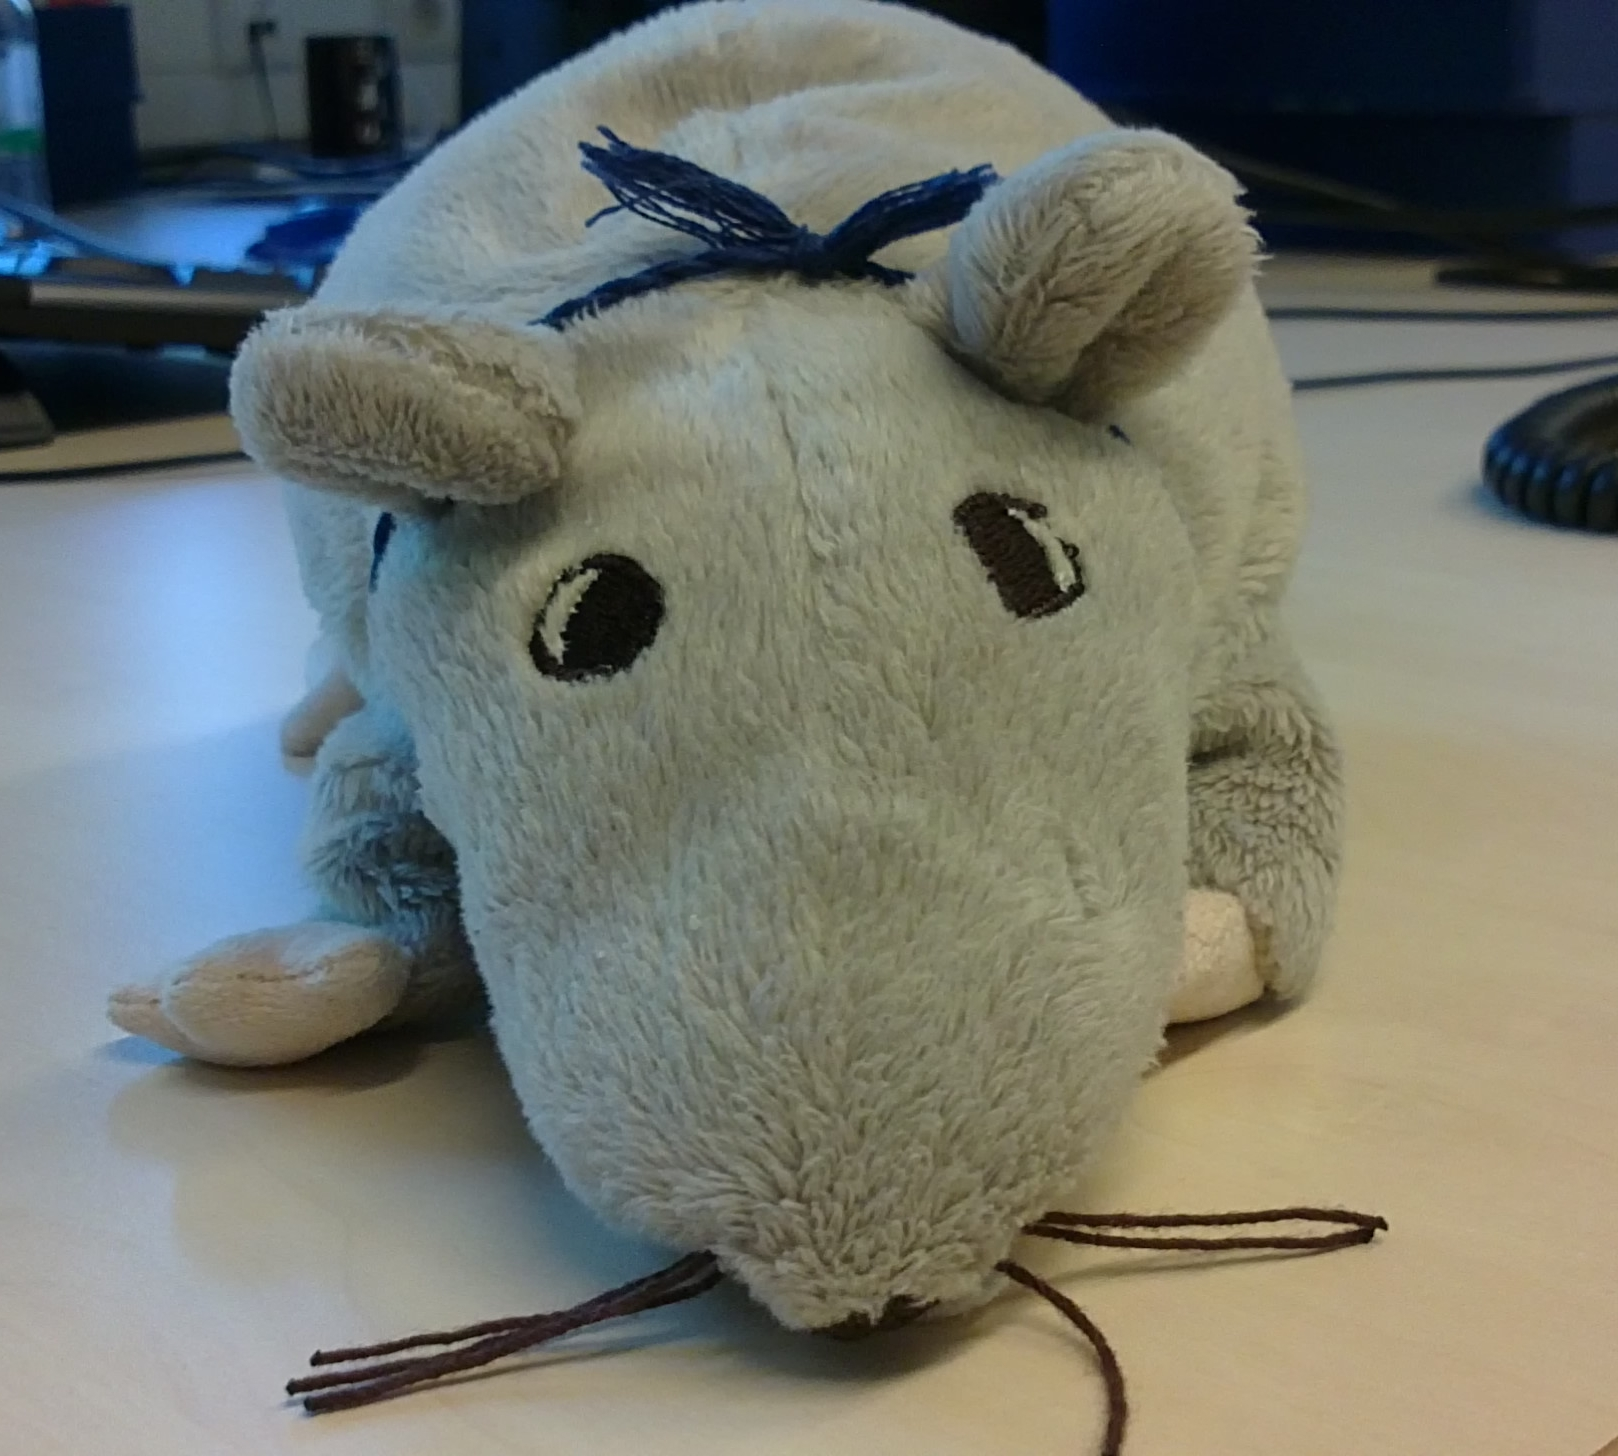
\includegraphics[width=0.8\linewidth]{pictures/ratte.jpg}
	\end{center}
	\caption{Proseminar supervisor's pet.}
	\label{fig:rat}
\end{figure}

\end{comment}